\section{Espaços métricos}

Na Proposição~\ref{prop:distanciaRn}, vimos que a distância usual de $\mathbb R^n$ satisfaz algumas propriedades básicas típicas do que se espera que uma noção de distância possua.
O conceito de espaço métrico consiste em nada mais do que um conjunto $M$ munido de uma função $d$ que satisfaz exatamente aquelas propriedades.

\begin{definition}\index{espaço métrico}\index{métrica}
    Seja $M$ um conjunto não vazio.
    Uma \emph{métrica} em $M$ é uma função $d:M\times M\to \mathbb R$ que satisfaz, para todos $p,q,r\in M$, as seguintes propriedades:
    \begin{enumerate}[label=(\roman*)]
        \item $d(p,q)\geq 0$, e $d(p,q)=0$ se, e somente se, $p=q$;
        \item $d(p,q)=d(q,p)$;
        \item $d(p,r)\leq d(p,q)+d(q,r)$.
    \end{enumerate}
    Um \emph{espaço métrico} é um par $(M,d)$, em que $M$ é um conjunto não vazio e $d$ é uma métrica em $M$.
\end{definition}

Quando $M=\mathbb R^n$ e $d$ é a distância Euclidiana, obtemos o principal exemplo deste texto.

A seguir, definiremos generalizações da noção de intervalo aberto de $\mathbb R$, conceitos essenciais para o futuro estudo de limite, continuidade e diferenciabilidade.

\begin{definition}\index{bola aberta}\index{bola|see{bola aberta}}\index{bola fechada}
    Sejam $(M,d)$ um espaço métrico, $p \in M$ e $r>0$.
    A \emph{bola aberta} de centro $p$ e raio $r$ é o conjunto:
    \begin{equation*}
        B_M(p, r) = \{q \in M : d(p, q) < r\}.
    \end{equation*}
    A \emph{bola fechada} de centro $p$ e raio $r$ é o conjunto:
    \begin{equation*}
        \overline{B}_M(p, r) = \{q \in M : d(p, q) \leq r\}.
    \end{equation*}
    Quando o espaço métrico estiver claro pelo contexto, escreveremos simplesmente $B(p,r)$ e $\overline{B}(p,r)$.
\end{definition}

No caso particular de $\mathbb R^n$, com a distância Euclidiana, uma bola aberta de raio $r$ centrada em $p$ é ilustrada abaixo.
\begin{figure}[H]
    \centering
    \begin{tikzpicture}
    \draw[->,ultra thick] (-4,0)--(4,0) node[right]{$x$};
    \draw[->,ultra thick] (0,-4)--(0,4) node[above]{$y$};
    % Centro da bola
    \filldraw[black] (2,2) circle (2pt);
    \node[below right] at (2,2) {$p$};
    % Raio da bola
    \draw[dashed] (2,2) circle (1.5);
    % Desenho do raio da bola
    \draw[-,thick] (2,2) -- (3.5,2) node[above right]{$r$};
    \end{tikzpicture}
    \caption{Bola aberta de centro $p$ e raio $r$ em $\mathbb R^2$.}
\end{figure}

Em $\mathbb R$, a bola aberta de centro $p$ e raio $r$ é exatamente o intervalo aberto $(p-r, p+r)$, como ilustrado abaixo.

\begin{figure}[H]
    \centering
    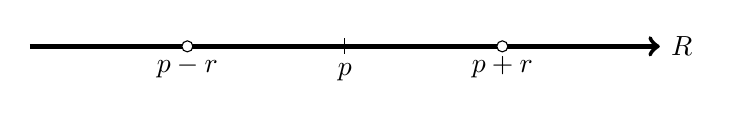
\begin{tikzpicture}
        % Eixo real
        \draw[->,ultra thick] (-4,0)--(4,0) node[right]{$\mathbb R$};
        % Intervalo aberto (p-r, p+r)
        \draw[thick] (-2,0) -- (2,0);
        % Pontos abertos nas extremidades
        \draw[fill=white] (-2,0) circle (2pt) node[below]{$p - r$};
        \draw[fill=white] (2,0) circle (2pt) node[below]{$p + r$};
        % Centro p
        \draw (0,0.1) -- (0,-0.1) node[below]{$p$};
    \end{tikzpicture}
    \caption{Bola aberta de centro $p$ e raio $r$ em $\mathbb R$.}
\end{figure}
